% Chương 2: Cơ sở lý thuyết

\chapter{Cơ sở lý thuyết}

% Trình bày cơ sở lí thuyết, các khái niệm và công nghệ chính sử dụng trong đề tài

\section{Apache Kafka}

Apache Kafka là một nền tảng xử lý luồng sự kiện phân tán được thiết kế để xử lý lưu lượng dữ liệu lớn với độ trễ thấp. Kafka hoạt động theo mô hình publish-subscribe, trong đó các producer gửi dữ liệu vào các topic, và các consumer đọc dữ liệu từ các topic này. Kafka được sử dụng rộng rãi nhờ khả năng mở rộng cao, độ bền vững và khả năng chịu lỗi.

Kiến trúc của Kafka bao gồm Producer (gửi dữ liệu), Broker (lưu trữ dữ liệu), Topic (danh mục logic), Partition (phân vùng để xử lý song song), và Consumer (đọc dữ liệu). Kafka sử dụng cơ chế offset để theo dõi vị trí đọc, đảm bảo consumer có thể đọc lại dữ liệu hoặc tiếp tục từ vị trí cũ khi xảy ra lỗi.

Trong đề tài này, Kafka làm hàng đợi tin nhắn giữa tầng thu thập và xử lý với ba topic: tiktok-raw, youtube-raw, và news-raw. Producer thu thập dữ liệu từ các nguồn và gửi vào topic tương ứng. Consumer đọc từ Kafka để xử lý qua pipeline phát hiện xu hướng.

\section{Apache Spark}

Apache Spark là framework xử lý dữ liệu lớn mã nguồn mở, hỗ trợ xử lý batch và streaming. PySpark là API Python của Spark. Ưu điểm lớn nhất của Spark là tốc độ xử lý nhờ in-memory computing thay vì đọc ghi đĩa như MapReduce. Spark cung cấp thư viện cho machine learning (MLlib), xử lý đồ thị (GraphX), và streaming.

Spark sử dụng kiến trúc master-worker với Driver Program (điều phối công việc), Cluster Manager (quản lý tài nguyên), và Executor (thực thi task). Spark sử dụng RDD (Resilient Distributed Dataset) - tập dữ liệu phân tán chịu lỗi, và cung cấp DataFrame/Dataset API với Catalyst Optimizer để tối ưu hiệu suất.

Trong đề tài này, PySpark xử lý batch dữ liệu từ Kafka. Consumer đọc từ ba topic, chuyển thành DataFrame, và xử lý qua pipeline tám giai đoạn. Spark xử lý hàng nghìn nội dung hiệu quả với xử lý song song. Hệ thống chạy local[*] để dùng tất cả core CPU.

\section{Vector Embeddings}

Vector embeddings là kỹ thuật biểu diễn văn bản dưới dạng vector số học trong không gian đa chiều (128-1536 chiều). Văn bản có ý nghĩa tương tự sẽ có vector gần nhau. Khoảng cách giữa hai vector (cosine similarity hoặc Euclidean distance) phản ánh mức độ tương đồng ngữ nghĩa.

Embeddings được tạo bởi các mô hình học sâu huấn luyện trên dữ liệu lớn, học cách nắm bắt ngữ nghĩa và ngữ cảnh. Ví dụ: "xe hơi" và "ô tô" có vector gần nhau vì cùng ý nghĩa, còn "xe hơi" và "máy bay" xa hơn dù cùng lĩnh vực giao thông.

Trong đề tài này, vector embeddings then chốt cho phân cụm và Gộp xu hướng. Hệ thống dùng OpenAI (text-embedding-3-small, 1536 chiều) hoặc Gemini để chuyển văn bản (nội dung + hashtags) thành vector. Vector này làm đầu vào cho HDBSCAN phân cụm nội dung tương đồng. Ở giai đoạn Gộp xu hướng, hệ thống tính cosine similarity giữa embedding xu hướng mới và cũ để quyết định có gộp hay không.

\section{HDBSCAN}

HDBSCAN (Hierarchical Density-Based Spatial Clustering of Applications with Noise) là thuật toán phân cụm dựa mật độ, cải tiến của DBSCAN. HDBSCAN phát hiện các cụm có mật độ khác nhau và tự động xác định số lượng cụm, khác k-means cần chỉ định trước.

Ưu điểm: (1) không cần chỉ định số cụm; (2) phát hiện cụm hình dạng bất kỳ; (3) xử lý tốt outliers (gán nhãn -1); (4) hoạt động với cụm mật độ khác nhau. Độ phức tạp O(n log n), cao hơn k-means nhưng chấp nhận được.

HDBSCAN hoạt động qua: (1) Xây đồ thị khoảng cách tối thiểu; (2) Tạo phân cấp cụm; (3) Trích xuất cụm ổn định; (4) Gán nhãn (cụm hoặc nhiễu -1). Tham số quan trọng là min\_cluster\_size (kích thước tối thiểu cụm).

Trong đề tài này, HDBSCAN phân cụm nội dung có embedding tương đồng thành xu hướng. Cấu hình: min\_cluster\_size=15, metric="euclidean", cluster\_selection\_method="eom". Hệ thống dùng two-pass clustering: lần đầu phân cụm, lần hai gán điểm nhiễu vào cụm gần nhất để tránh bỏ sót nội dung tiềm năng.

\begin{figure}[H]
    \centering
    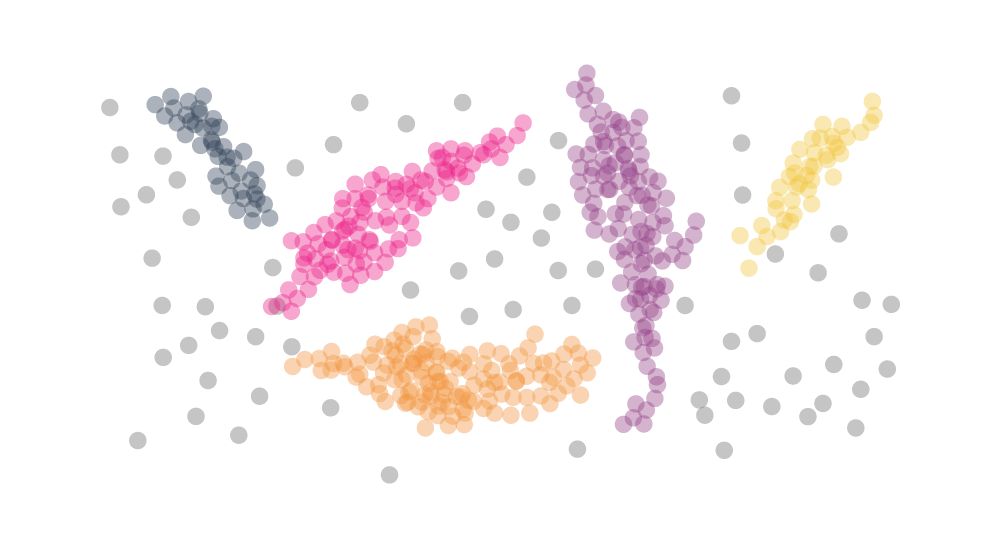
\includegraphics[width=0.8\textwidth]{images/hdbscan.png}
    \caption{Minh họa thuật toán HDBSCAN phân cụm dựa mật độ}
    \label{fig:hdbscan}
\end{figure}

\section{Large Language Models}

Large Language Models (LLM) là mô hình ngôn ngữ lớn huấn luyện trên dữ liệu văn bản khổng lồ, có khả năng hiểu và sinh văn bản tự nhiên. LLM dùng kiến trúc Transformer với hàng tỷ tham số, thực hiện nhiều tác vụ NLP như tóm tắt, phân tích cảm xúc, trích xuất thông tin, dịch máy.

LLM phổ biến: gpt-4.1-mini (OpenAI), Gemini (Google), Claude (Anthropic), Llama (mã nguồn mở). Ưu điểm là few-shot và zero-shot learning, chỉ cần mô tả tác vụ bằng ngôn ngữ tự nhiên (prompt engineering).

Trong đề tài này, LLM dùng cho: (1) Embedding - OpenAI text-embedding-3-small hoặc Gemini chuyển văn bản thành vector 1536 chiều cho phân cụm và Gộp xu hướng; (2) Phân tích xu hướng - gpt-4.1-mini hoặc Gemini phân tích từng cụm. Với mỗi cụm, hệ thống chọn top 10 nội dung engagement cao, xây prompt và yêu cầu LLM trích xuất: topic, summary, sentiment, keywords, content\_type, risk\_level, guidelines cho marketer/social manager. LLM cho phép phân tích tự động mà không cần rules thủ công.
